\documentclass{beamer}
%\usetheme{Ilmenau}
%\usecolortheme{beaver}

\usepackage[slovak,american]{babel}
\usepackage[utf8]{inputenc}
\usepackage{graphicx}
\usepackage{adjustbox}
 \usepackage{xcolor}
 
 \newsavebox\MBox
\newcommand\Cline[2][red]{{\sbox\MBox{$#2$}%
  \rlap{\usebox\MBox}\color{#1}\rule[-2.2\dp\MBox]{\wd\MBox}{1pt}}}

%\usefonttheme{serif}

\definecolor{UKOrange}{HTML}{ef9424} %
\definecolor{UKBrown}{HTML}{a96d5e} %
\definecolor{UKLight}{HTML}{d8b6ab} %
\definecolor{UKDark}{HTML}{7a4f44}
\definecolor{UKDarker}{HTML}{4d312b} 
\definecolor{UKDarkest}{HTML}{2e1e1a}
\definecolor{UKRed}{HTML}{bf1f1c}

\setbeamertemplate{footline}[frame number]{}
\setbeamertemplate{navigation symbols}{}

%\usecolortheme{beaver}
\setbeamertemplate{itemize item}[square]
\setbeamercolor{itemize item}{fg = UKBrown}
\setbeamercolor{itemize subitem}{fg = UKLight}
\setbeamercolor{enumerate item}{fg = UKDark}

\setbeamercolor{footnote}{fg=UKLight}
\setbeamercolor{footnote mark}{fg=UKLight}
\setbeamerfont{footnote}{size=\tiny}
\renewcommand\footnoterule{}

\usetheme{default}
\beamertemplatenavigationsymbolsempty
\setbeamercolor{title}{fg=white, bg=UKBrown}
\setbeamercolor{frametitle}{fg=white, bg=UKBrown}
\setbeamercolor{block title}{bg=UKBrown, fg= white}
\setbeamercolor{block body}{bg =UKLight, fg = UKDarkest}

\useoutertheme[subsection=false]{miniframes}
\AtBeginSection[]{\subsection{}}

\setbeamercolor{below lower separation line head}{bg=UKDark}
\addtobeamertemplate{headline}{}{%
  \begin{beamercolorbox}[colsep=0.5pt]{below lower separation line head}
  \end{beamercolorbox}
}
%\setbeamercolor*{mini frame}{fg=white,bg=UKRosy}
\setbeamercolor{section in head/foot}{fg=UKLight, bg=UKDark}

%\setbeamertemplate{itemize/enumerate body begin}{\normalsize}
%\setbeamertemplate{itemize/enumerate subbody begin}{\normalsize}




%\newcommand{\codeblock}[2]{ \begin{block}{#1} \begin{verbatim}#2\end{verbatim}\end{block}}

%\defbeamertemplate*{title page}{customized}[1][]
%{
%  \begin{centering}
%    \begin{beamercolorbox}[sep=8pt,center]{title}
%      \usebeamerfont{title}\inserttitle
%    \end{beamercolorbox}
%  \end{centering}
%  \bigskip
%
%\begin{columns}[onlytextwidth,T]
%
%
%  \column{27mm}
%  \includegraphics[width=27mm]{images/logoFMFI.png}
%  
%  \column{\dimexpr\linewidth-54mm-6mm}
%  \centering
%  \vspace{5mm}  
%  \usebeamerfont{author}\insertauthor\par
%  \vspace{5mm}
%  \usebeamerfont{institute}\insertinstitute\par
%
%  \column{27mm}
%  \includegraphics[width=27mm]{images/logoUK.png}  
%\end{columns}
%\centering
%\vspace{7mm}
%  \usebeamerfont{date}\insertdate\par
%}


\title[kNN]{Rozpoznávanie obrazcov - 7th lab \\ kNN and validation}
\author[Viktor Kocur]{Viktor Kocur \\{\small viktor.kocur@fmph.uniba.sk}}
\institute{DAI FMFI UK}
\date{6.4.2019}
%\titlegraphic{\includegraphics[width=2.7cm]{images/logoFMFI.png}\hspace*{1cm}~%
%   \includegraphics[width=2.7cm]{images/logoUK.png}
%}


\begin{document}
\selectlanguage{american}

\begin{frame}[plain]
  \titlepage  
\end{frame}

\section{k nearest neighbors}

\begin{frame}
\frametitle{k nearest neighbors}
\begin{block}{Basics}
In the feature space $\mathbb{R}^n$ with a metric $\rho$ we can choose a class for a feature vector $\vec{x} \in \mathbb{R}^n$ by finding its $k$ nearest neighbors from the training set and select the class which has the most members from the $k$ neighbors. 
\end{block}

\begin{block}{Training}
This method does not need training. The method always takes the whole training set and looks for neighbors. With large training set this method can be slow.
\end{block}
\end{frame}


\begin{frame}
\frametitle{Metric functions}
\begin{block}{Definition}
Let $P$ be a set. Then a metric is a function $\rho: P \times P \mapsto \mathbb{R}_0^+$ such that $\forall p, q, r \in P$: \\
1. $\rho(p,q) \ge 0$ \\
2. $\rho(p,q) = 0 \Leftrightarrow p = q$ \\
3. $\rho(p,q) = \rho(q,p)$ \\
4. $\rho(p,r) \leq \rho(p,q) + \rho(q,r)$\\
\vspace{1em}
A set with a metric is also called a metric space.
\end{block}
\end{frame}


\begin{frame}
\frametitle{Metrics}
\begin{block}{Metrics on $\mathbb{R}^n$}
$$\rho_e(\vec{x}, \vec{y}) = \sqrt{\sum_{i = 1}^n (x_i - y_i)^2 }   $$
$$\rho_m(\vec{x}, \vec{y}) = \sum_{i = 1}^n |x_i - y_i |   $$
$$\rho_q(\vec{x}, \vec{y}) = \left( \sum_{i = 1}^n (x_i - y_i)^q  \right)^{\frac{1}{q}} $$
$$\rho_{max}(\vec{x}, \vec{y}) = max_{i} | x_i - y_i |  $$
\end{block}
\end{frame}


\begin{frame}
\frametitle{Choosing k}
\center
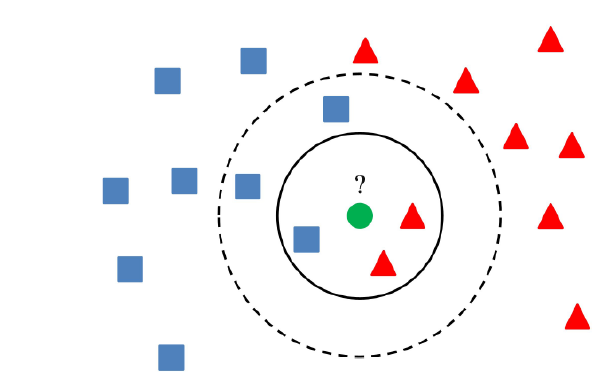
\includegraphics[width=0.8\textwidth]{knn2.png}
\end{frame}

\begin{frame}
\frametitle{Choosing k}
\center
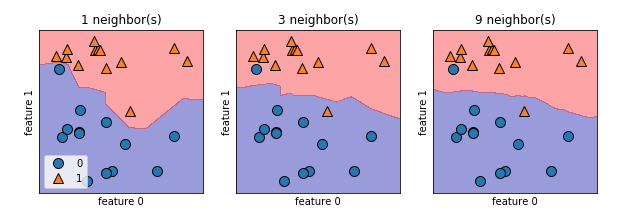
\includegraphics[width=1.1\textwidth]{knn.png}
\end{frame}


\begin{frame}
\frametitle{Exercise}
\begin{block}{Exercise}
Create a function mykNN(k, X, y, p) which returns class for a vector p based on training data X with classes y.
\end{block}

\begin{block}{Exercise}
Test the function on the data from the last lab and the fisheriris database.
\end{block}
\end{frame}

\begin{frame}
\frametitle{Exercise}
\begin{block}{fitcknn}
Mdl = fitcknn(X,y) - creates a kNN classifier
\end{block}

\begin{block}{predict}
Mdl.predict(x) - retursn kNN model prediction
\end{block}

\begin{block}{Properties}
Interesting properties are: 'Standardize', 'Distance', 'NumNeighbors', 'NSMethod'. Check them in help.
\end{block}

\begin{block}{Exercise}
Change the m-file for displaying the SVM classifier from the previous lab and show the boundaries for kNN.
\end{block}
\end{frame}


\section{Validation}
\begin{frame}
\frametitle{Data split}
\begin{block}{Training set}
So far we have only used only the training set. All of the data we had were used to find the parameters of the model.
\end{block}

\begin{block}{Test set}
In case we want to verify that our model is reliable it is important to leave some of the data for testing. The testing data are only used at the very end our research when our model is ready. The test set is used to verify the model. You should never use the training set to select the method, its parameters or hyperparameters.
\end{block}
\end{frame}


\begin{frame}
\frametitle{Data split}
\begin{block}{Validation set}
Since the test set cannot be used to choose the model we need one more set for this purpose. The validation set is used to determine the correct approach and finding the optimal hyperparameters of the model.
\end{block}

\begin{block}{Data split}
We split the data based on their amount, properties and models. Huge amounts of data are required for neural networks, therefore a split can be 80/10/10. With some other methods a split of 60/20/20 is good enough. In some cases the spil can be even 40/20/40.
\end{block}
\end{frame}


\begin{frame}
\frametitle{Validation}
\begin{block}{Hyperparameters}
We can determine the correct hyperparameters on the validation. Hyperparameters are the settings/parameters, which affect how the model is trained or how the prediction works. Hyperparameters for SVM include the kernel type and scale. For kNN it can be the choice of $k$ and the metric used.
\end{block}

\begin{block}{Validation}
We perform validation by training the model (for kNN just creating it) on the the training set with different hyperparameters. These models are then tested on the validation set. We select a reliability metric, ideally classification accuracy. Based on the results we choose the hyperparameters which achieved the best results.
\end{block}
\end{frame}



\begin{frame}
\frametitle{Validation - exercise}
\begin{block}{Exercise}
Split the data from the previous lab into train/val/test split of 60/20/20. Choose the best $k$ parameter for the kNN classifier and a metric on the validation split.
\end{block}

\begin{block}{Proper representation}
Some datasets are ordered by class or occur in some othe regular order. It is therefore necessary to verify that the split is meningful. Ideally we would keep the same ratio of classes for all sets.
\end{block}
\end{frame}

\begin{frame}[fragile]
\frametitle{Crossvalidation}
\begin{block}{Crossvalidation}
If we only have very little data we do not split it into the training and validation sets. The data are split into $n$ approximately similar subsets. We train the model on all except one of the subsets and test it on the remaining set. We repeat this $n$ times for all the subsets and average out the results.
\end{block}

\begin{block}{Matlab}
\begin{verbatim}
Mdl = fitcknn(X, y, 'NumNeighbors', k);
CVMdl = crossval(Mdl)
loss = kfoldLoss(CVMdl) \end{verbatim}
\end{block}
\end{frame}



\begin{frame}[fragile]
\frametitle{Crossvalidation}
\begin{block}{Automatic selection of hyperparameters}
For most of the fitc.. functions it is possible to let Matlab select the hyperparameters automatically. Check help if you want to use this feature.
\end{block}

\begin{block}{Matlab}
\begin{verbatim}
Mdl = fitcknn(X,Y,'OptimizeHyperparameters','auto')\end{verbatim}
\end{block}
\end{frame}
\end{document}